
\teaser{
\centering
\vspace{-6pt}
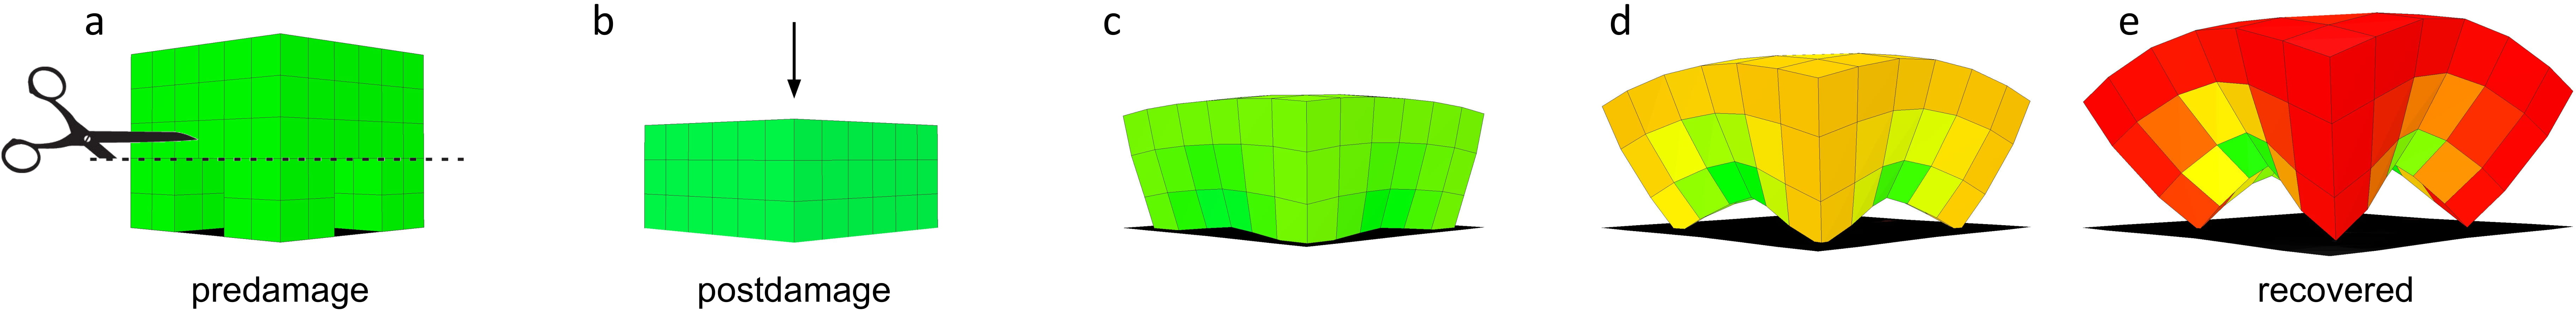
\includegraphics[width=\linewidth]{fig/bigger_teaser.jpg} \\
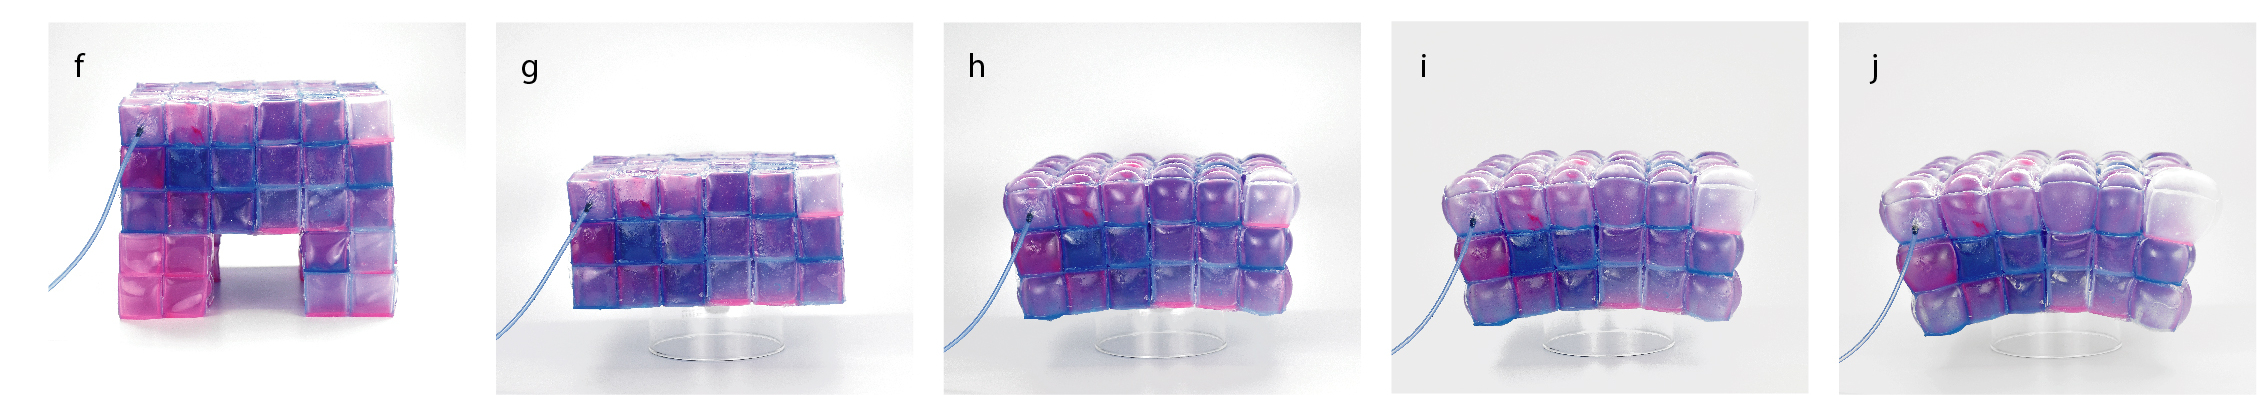
\includegraphics[trim={0 0 0 4pt},clip,width=\linewidth]{fig/VoxelBotCropped.jpg} \\
\vspace{-4pt}
\caption{After learning to walk, a simulated quadruped is subjected to unanticipated insult: its legs are cut off. 
An evolutionary algorithm searches for deformations to the postdamage structure that, when coupled with the predamage controller, result in function recovery.
One of the evolved solutions (shown here) yields the spontaneous ``regeneration'' of the lost legs, which was manually transferred to reality (\href{https://youtu.be/afOXX2r54mQ}{\textcolor{blue}{\textbf{\texttt{youtu.be/afOXX2r54mQ}}}}).
} 
\label{fig:teaser}
\vspace{-20pt}
}


